\documentclass[a4paper]{article}

\usepackage[T1]{fontenc}
\usepackage[adobe-utopia]{mathdesign}
\usepackage[protrusion=true,expansion=true]{microtype}
\usepackage{xcolor}

\definecolor{darkblue}{rgb}{0,0,0.5}

\usepackage[colorlinks=true,
        urlcolor=darkblue,
        anchorcolor=darkblue,
        linkcolor=darkblue,
        citecolor=darkblue,
        pdfauthor={Tarek Fouda},
        pdfkeywords={educational tools, pseudo-code, virtual machine,
          parser, interpreter},
        pdftitle={Pseudo-code virtual machine},
        pdfsubject={Bachelor topic proposal for the faculty for MET,
          the German University in Cairo GUC
          (http://met.guc.edu.eg/)}]{hyperref}
\usepackage{url}

\author{Tarek Fouda}
\title{Pseudo-code virtual machine. First Interim report}

\begin{document}

\maketitle

\begin{abstract}
  $ Pseudo code $ -- First year students who are newly introduced to the idea of coding and algorithms face a lot of problems during understanding the mechanics of a simple Pseudocode algorithm as they do not see an output to what they run and they do not have a feedback on their code except with the grades on the assignments and quizzes. We thought of creating a tool that would help such new students to fully understand the concept and the flow of a code, mainly this tool is a visualizing interpreter for a modified pseudo-code, that allows entering, editing, and step-by-step executing of mini-code while observing the effects of statements and control-flow as they happen.
  
  
  \end{abstract}
  \bigskip
  \bigskip
  

To begin with this tool we should understand what a compiler is and what it does. A compiler is a program that translates a source program written in some high-level programming language (In our task the programming language is Pseudo Code) into machine code for some computer architecture. The generated machine code can be later executed many times against different data each time. Interpreters are not much different than compilers. They also convert the high level language into machine readable binary equivalents. Each time when an interpreter gets a high level language code to be executed, it converts the code into an intermediate code before converting it into the machine code. Each part of the code is interpreted and then execute separately in a sequence and an error is found in a part of the code it will stop the interpretation of the code without translating the next set of the codes. The only difference between them is that interpreters take one statement then translate it executes it and then takes another statement. While the compiler translates the entire program in one go and then executes it.Compiler generates the error report after the translation of the entire page while an interpreter will stop the translation after it gets the first error.
·         Compiler takes a larger amount of time in analyzing and processing the high level language code comparatively interpreter takes lesser time in the same process.
·         Besides the processing and analyzing time the overall execution time of a code is faster for compiler relative to the interpreter.

Thanks to Engineers garage for stating this comparison.

\newpage
\bigskip
  \bigskip

It was decided we were going to use Java programming language for this task. There are a lot of Java parser generators (Antlr, JavaCC, BYACC/J ..etc) but we had to pick a specific one.

One major difference is that ANTLR generates an LL(*) parser, whereas YACC and Bison both generate parsers that are LALR. This is an important distinction for a number of applications, the most obvious being operators:
\\*
\\*
expr ::= expr '+' expr
       | expr '-' expr
       | '(' expr ')'
       | NUM ;
       \\*
\\*


ANTLR is entirely incapable of handling this grammar as-is. To use ANTLR (or any other LL parser generator), you would need to convert this grammar to something that is not left-recursive. However, Bison has no problem with grammars of this form. You would need to declare '+' and '-' as left-associative operators, but that is not strictly required for left recursion. A better example might be dispatch:
\\*
\\*
expr ::= expr '.' ID '(' actuals ')' ;
\\*
actuals ::= actuals ',' expr | expr ;
\\*
\\*
Notice that both the expr and the actuals rules are left-recursive. This produces a much more efficient AST when it comes time for code generation because it avoids the need for multiple registers and unnecessary spilling (a left-leaning tree can be collapsed whereas a right-leaning tree cannot).

In terms of personal taste, I think that LALR grammars are a lot easier to construct and debug. The downside is you have to deal with somewhat cryptic errors like shift-reduce and (the dreaded) reduce-reduce. These are errors that Bison catches when generating the parser, so it doesn't affect the end-user experience, but it can make the development process a bit more interesting. ANTLR is generally considered to be easier to use than YACC/Bison for precisely this reason.So we settled down on using Antlr as the parser generator of this task. \\
\\*
Installing Antlr is pretty easy. www.antlr.org introduces simple steps for installing Antlr for Windows or Unix users.

\begin{figure}[h!]
\centering
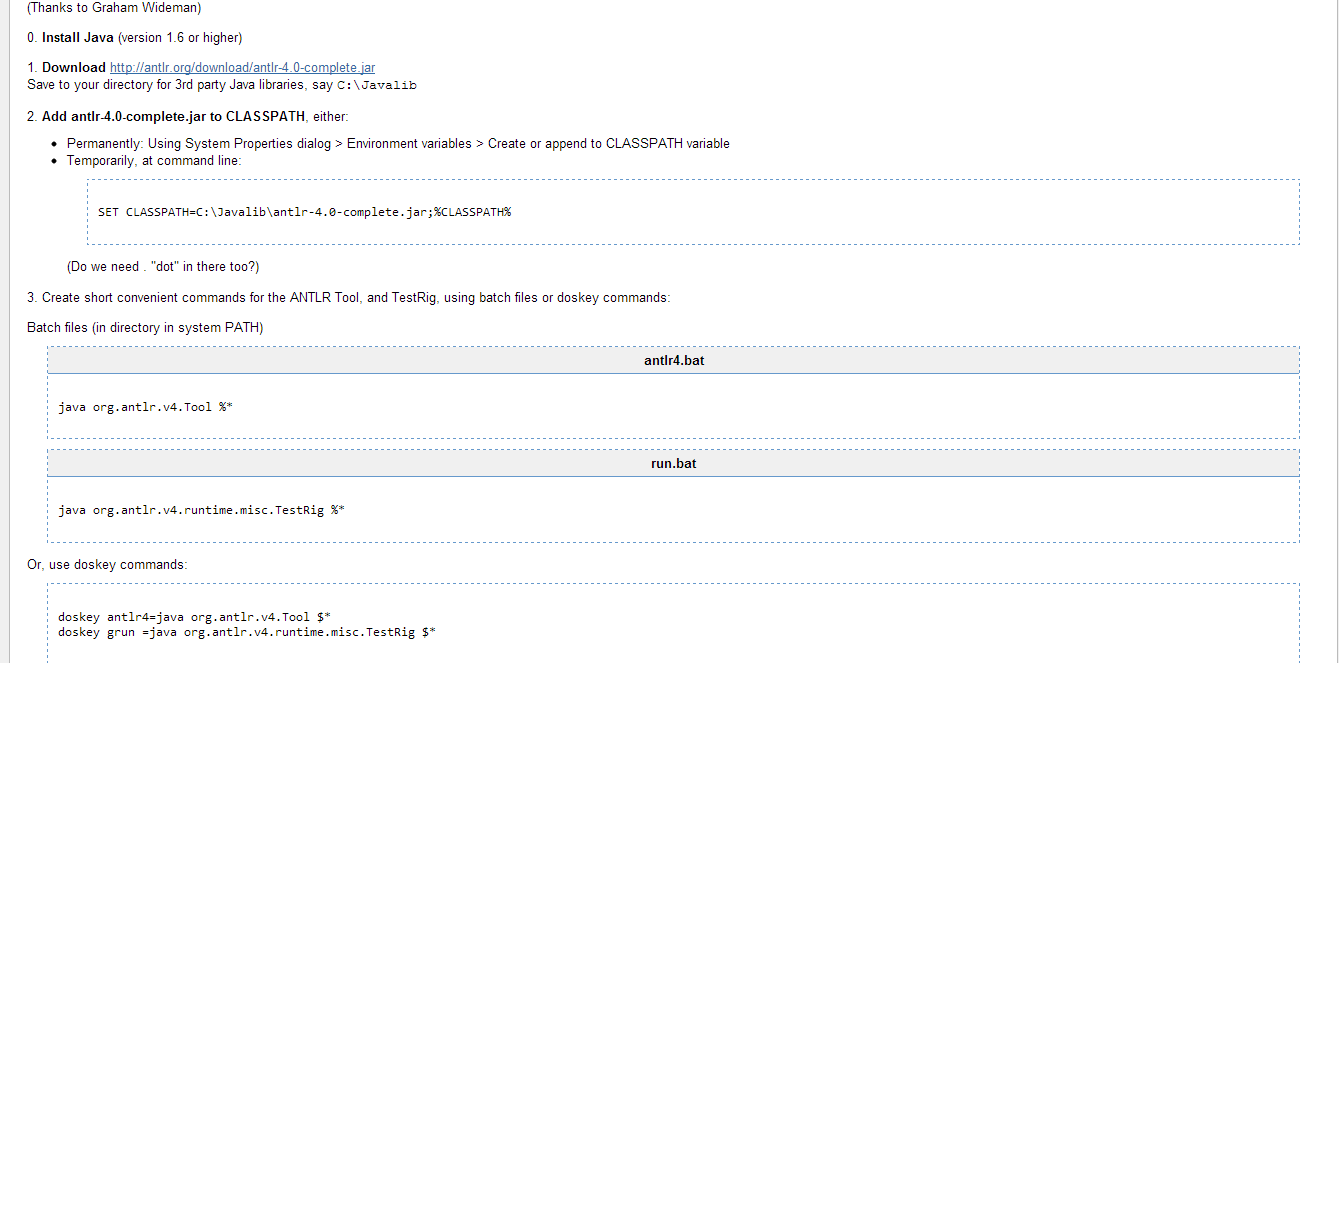
\includegraphics{report1.png}
\caption{The Universe}
\label{threadsVsSync}
\end{figure}
 
The task requires implementing Graphic user Interface as a window the student types in the Pseudo-Code and presses a button to compile the piece of code and debug the code line by line, from this point we thought of integrating Antlr with eclipse to come up with such a tool and to enhance the infrastructure of the project.

Antlr IDE was required to be installed on eclipse. By installing Antlr IDE the grammar file had 3 views.

The first view of the grammar file was the grammar itself as shown in the figure below.
\begin{figure}[h!]
\centering
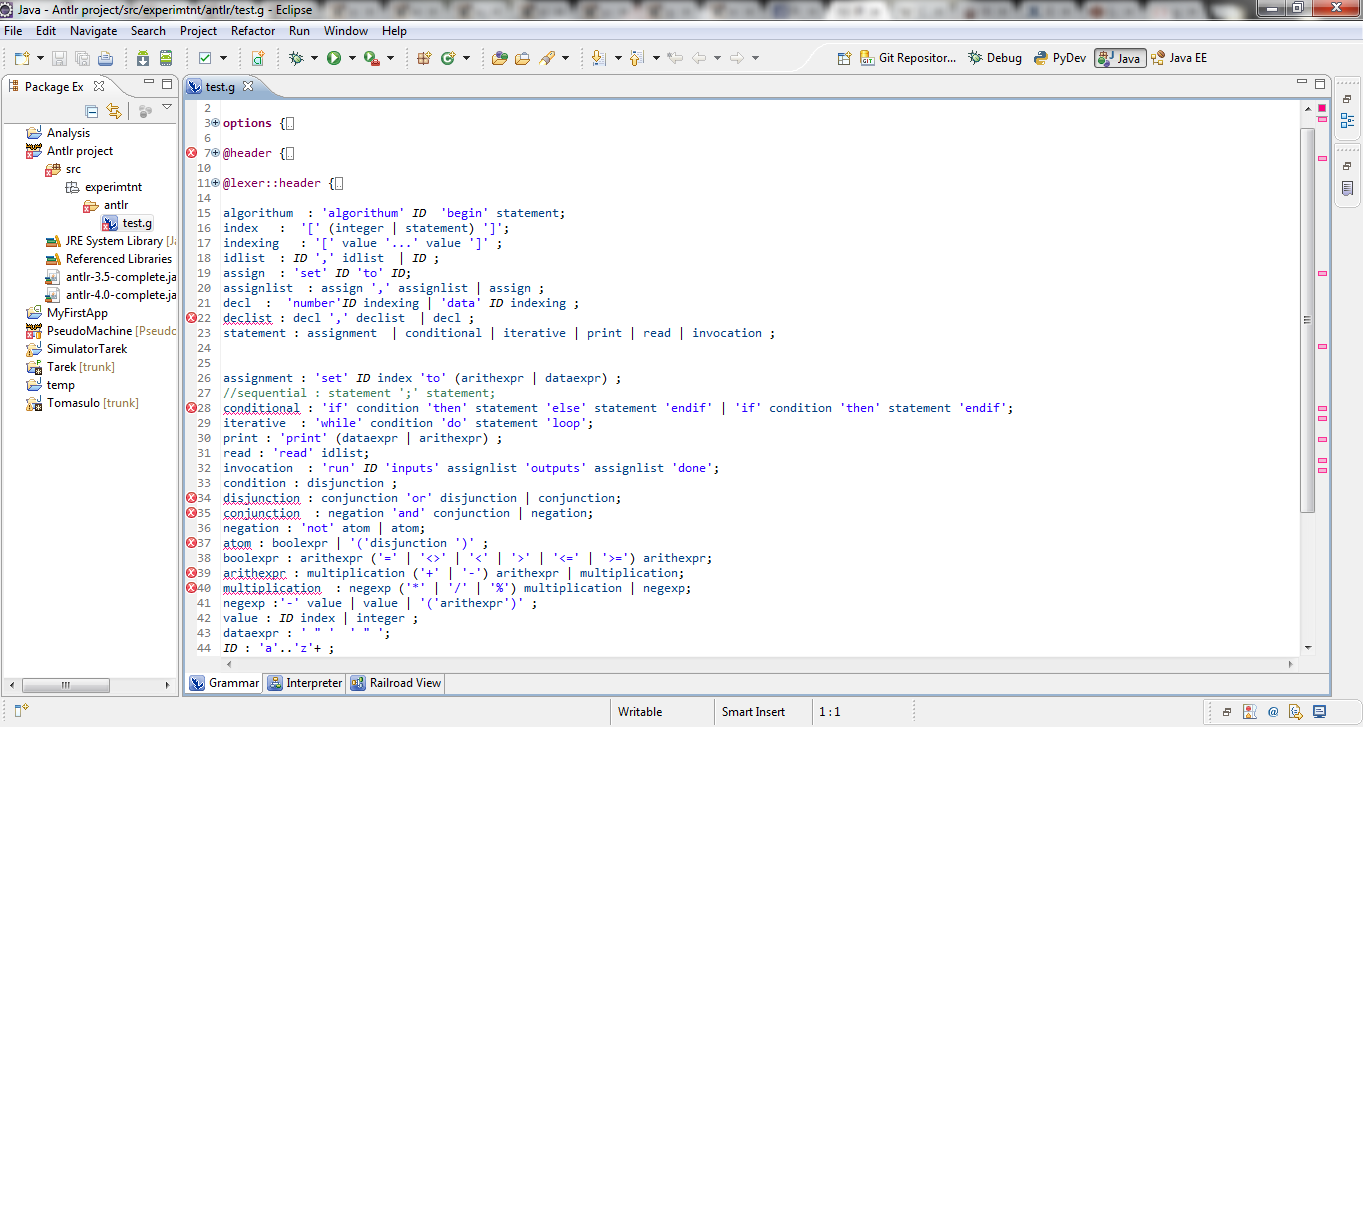
\includegraphics{report2.png}
\caption{Grammar view}
\label{threadsVsSync}
\end{figure}

\\*
The second view is the interpreter, you type in a sample algorithm and a simple graph is expected to be shown. The figure below illustrates the Interpreter view.

\begin{figure}[h!]
\centering
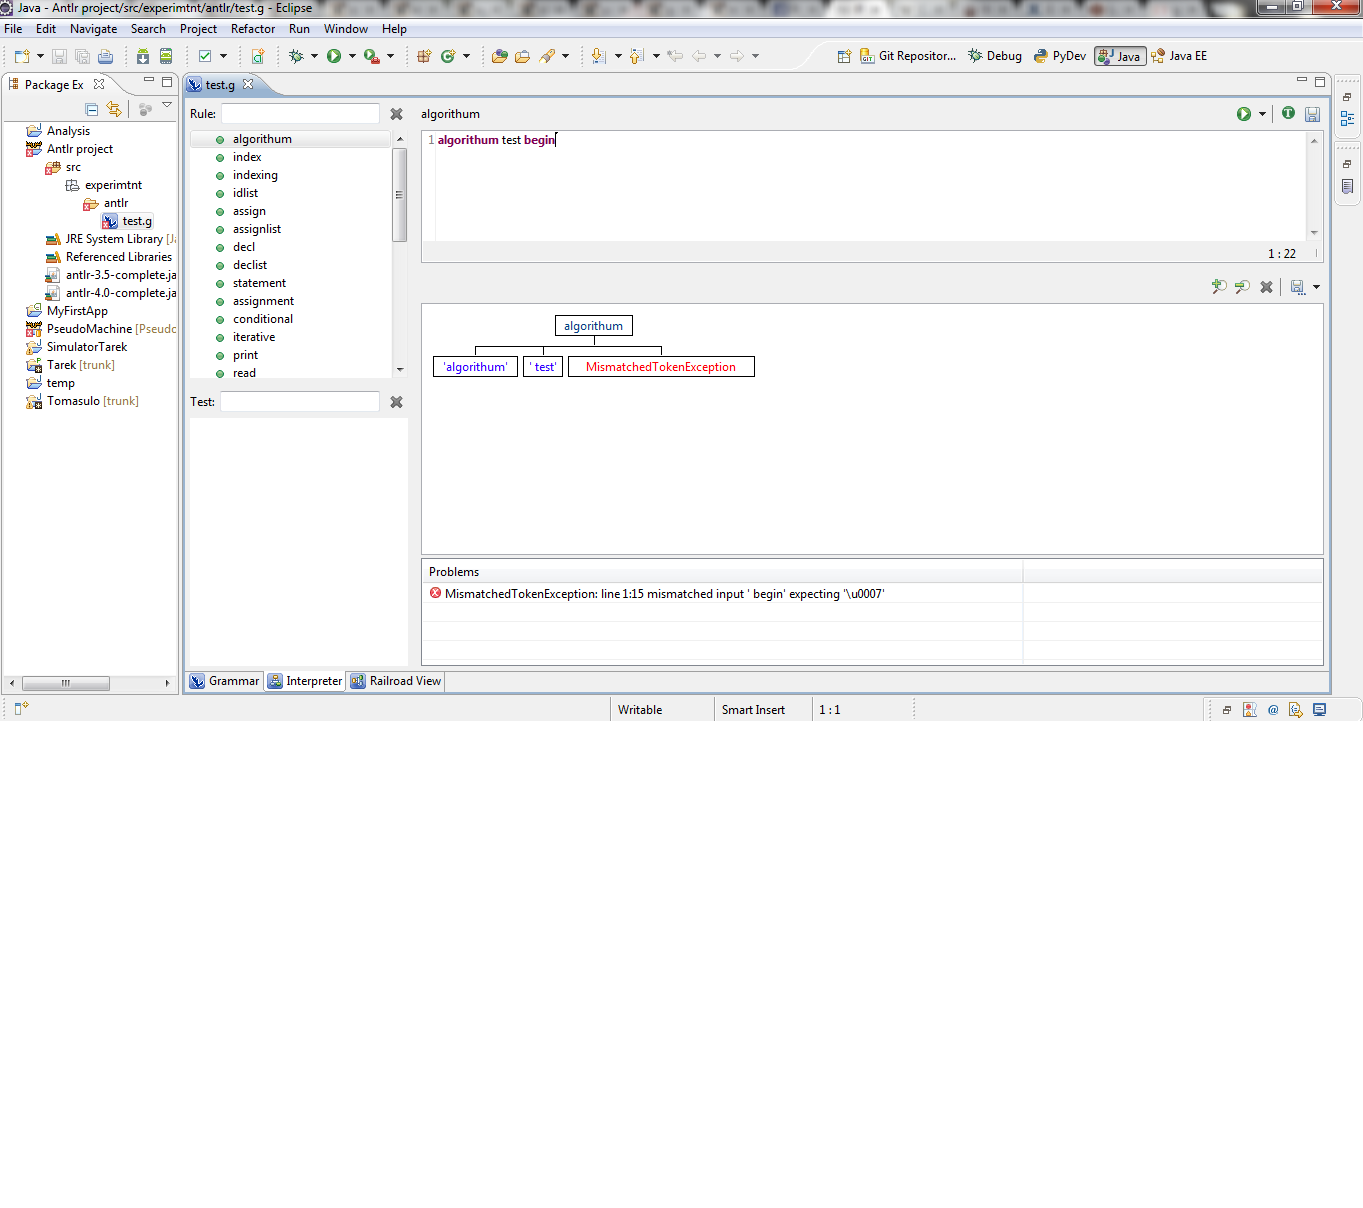
\includegraphics{report3.png}
\caption{Interpreter view}
\label{threadsVsSync}
\end{figure}

\\*

The third and the final view is the RailRoad view of the rules.

\begin{figure}[h!]
\centering
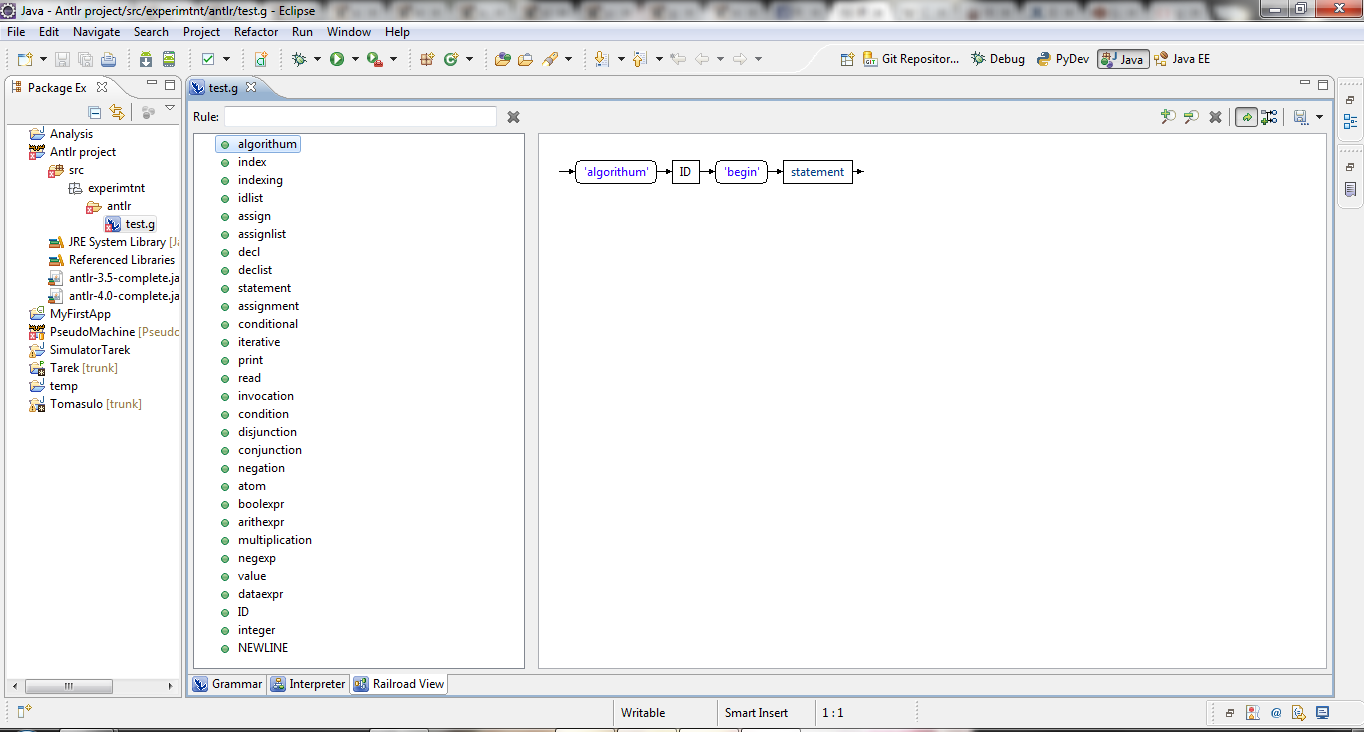
\includegraphics{report4.png}
\caption{RailRoad view}
\label{threadsVsSync}
\end{figure}



\end{document}

%%% Local Variables: 
%%% mode: latex
%%% TeX-master: t
%%% End: 

\begin{figure}[h!]
\centering
\includegraphics[scale=1.7]{universe.jpg}
\caption{The Universe}
\label{threadsVsSync}
\end{figure}


